\chapter{Background and Related Work}
\label{chap:background}

% \section{NAPLab Car}

\section{CARLA Simulator}
\acrfull{carla} is an open source photo-realistic simulator for autonomous driving research \cite{introducing-carla-paper}. It was developed from the ground up to support development, training and validation of autonomous urban driving systems. CARLA provides free open digital assets such as urban layouts, buildings and vehicles. Additionally the simulator includes a suit of sensors, environmental conditions, full control over of static and dynamic actors, a traffic manager and more.

CARLA is built with a scalable client-server architecture in mind. The server uses Unreal Engine \cite{unrealengine} as a simulation foundation and is responsible for tasks such as scene and sensor rendering, computation of realistic physics, actor updates and providing updated world information to the connected clients. Multiple clients can be connected to the CARLA server, and these send commands to the server and receive updated world information in return. Example commands are traffic generation, spawning new actors, controlling vehicles and setting weather conditions.

\subsection{Python API}
To implement the client-server functionality, the CARLA team has developed client APIs in Python \cite{carla-python-api} and C++ \cite{carla-cplusplus-api} that leverages sockets to establish a connection to the server. The work in this project is based on the latest released version of the Python API, which in the time of writing is version 0.9.13. The Python API can be used to control the core parts of the simulation: 

\begin{description}
    \item[World:] The world represents the simulation, and one can change properties such as weather conditions, lighting and the map to use.
    \item[Map:] The map represents the actual simulated world, often called the town. The client can manage roads, lanes and junctions in the map, which are used together with waypoints to provide vehicles with a navigation path. Waypoints are simply points in 3D space oriented in the direction of the lane containing it.
    \item[Actors:] An actor is anything that plays a role in the simulation. Examples are pedestrians, vehicles, sensors and traffic lights.
    \item[Blueprints:] Blueprints are already-made models used to spawn new actors into the world. These includes properties such as vehicle color, sensor channels and pedestrian walking speed.
    \item[Sensors:] Sensors are attached to vehicles. They observe the simulated environment, collect data and make this available to the client. Many sensor types exists in CARLA, including realistic sensors (cameras, \acrshort{lidar}, GPS, etc.) and ground-truth sensors from the simulator (collision detection, semantic segmentation, etc.). 
\end{description}


\subsection{Leaderboard}
The CARLA Autonomous Driving Leaderboard \cite{carla-leaderboard} is an open platform for evaluation of driving performance by autonomous agents in realistic traffic scenarios. The goal of the platform is to simplify comparisons between different approaches to autonomous driving using a set of predefined routes. The routes vary in weather conditions and world layouts, and contain scenarios such as lane merging, lane changing, intersections, yielding to emergency vehicles and handling traffic lights. They also have constraints on which type of sensors one can utilize, depending on which leaderboard track they belong to. There are two leaderboard tracks; the "SENSORS track" only allows access to sensors attached to the vehicles, while the "MAP track" allows access to an HD world map in addition to the sensors.

The evaluation is based on two metrics. The first is route completion, which simply is the average percentage of route distance completed. The other metric counts infractions per kilometer and aggregates them into a penalty score. The infraction types counted by the leaderboard are collisions with pedestrians, vehicles and static objects, as well as running red lights and stop signs. The route completion score and infraction score is combined into a driving score, which is the main metric of the leaderboard.

There are two versions of the leaderboard. Leaderboard 1.0 is for CARLA version 0.9.10, while Leaderboard 2.0 is for the latest CARLA version (0.9.13). Although Leaderboard 2.0 is the current version, it contains no entries at the time of writing. This report will therefore discuss submissions from Leaderboard 1.0.


\subsection{Alternatives to CARLA}
There exists multiple simulator alternatives to CARLA, each with their own advantages and disadvantages. They often have a trade-off between visual fidelity of the simulated 3D environment and the level of realism in the computed vehicle physics. According to \textcite{carla-an-inside-out}, who have done an extensive comparison between different alternatives, the state-of-the-art simulators that best meet this trad-off are CARLA and LGSVL \cite{LGSVL-simulator}. Similarly to CARLA, the open source LGSVL simulator provides tools which allows users to customizes sensors, controllable objects and other modules. Additionally, LGSVL provides integration with autonomous driving software which makes it a fully end-to-end tool. Note that the simulator stopped receiving updates by original authors as of January 2022. There still exist usable forks of the project which can be used, however. Other popular open source alternatives are AirSim \cite{airsim}, DeepDrive \cite{deepdrive} and Torcs \cite{torcs}.

An interesting upcoming simulator is NVIDIA Drive Sim \cite{nvidia-drive-sim}. It is an end-to-end simulation platform with focus on being physically accurate, fast and efficient at scale. While this is a project showing impressive photo realistic simulation, it is currently in an early access phase, meaning you need to apply to access it. Another disadvantage is the commercial and closed nature of the product, meaning that one will have less control and configurability over the simulator.

% kun CARLA finnes på paperswithcode

\section{Deep Learning}

Deep learning is a subset of machine learning that uses artificial neural networks to model complex patterns in data.
Artificial neural networks are high-dimensional non-linear mathematical functions
composed from common building blocks like
convolutions, matrix multiplications, and various non-linear functions.
In the context of self-driving vehicles,
deep learning algorithms can be used to analyze images and other sensory data to make decisions about how to navigate the environment.
Artificial neural networks can be trained using supervised, unsupervised, or reinforcement learning techniques,
depending on the specific problem and dataset.
In this section,
we will explore some of the key concepts and techniques used in deep learning for self-driving vehicles.

https://arxiv.org/abs/1704.05519  \cite{computer-vision-for-autonomous-vehicles}

https://ieeexplore.ieee.org/document/9700770 \cite{survey-on-end-to-end-techniques}


\subsection{Supervised learning}
\label{sec:superviser-learning}
% 90% literally written by chatgpt lmao 
Supervised learning is a type of machine learning algorithm witch utilizes a labeled dataset.
That is, the dataset consists of pairs of input and output data,
and the model is trained to predict the output ("label") given the input.
The goal of supervised learning is to make a model
capable of making predictions on new data
based on the patterns it learned from the training data.
In the case of self-driving vehicles,
the labeled data might consist of images and the corresponding steering angles for those images,
with the goal of the model being to predict the correct steering angle for new,
unseen images.

A common algorithm used in supervised learning is stochastic gradient descent.
The algorithm works by iteratively querying the model for a prediction given an input,
and then updating the model's parameters to reduce the error between the predicted output and the true label.
At each iteration, the algorithm computes the gradient of the error with respect to the model's parameters and uses this gradient to update the parameters in a direction that reduces the error.
This process is repeated until a satisfactory low error is achieved.


\subsection{Imitation Learning}

Imitation Learning (IL) learning is an approach to training autonomous agents
where the agents are trained to imitate the behaviour of an expert agent.
The expert agent is used to determine the best course of action $a$ when exposed to different states $s$,
which results in sequences of state-action pairs $(s, a)$.
These state-action pairs serve as the ideal action choices
that we wish to teach the imitating agent.
Within the IL regime,
there are three main algorithms for learning,
which we will explore in further detail.

Behavioural Cloning (BC) is one approach where the state-action pairs
are treated as inputs to a supervised learning algorithm.
Given an expert policy $\pi^*$ that one wishes to imitate,
first generate a dataset $\mathcal{D}$
with $N$ samples $\mathcal{D}_i = (s^*_i, a^*_i), i = 1 \dots N$
from the expert policy distribution $d^{\pi^*}$.
Then, using supervised learning,
recover an approximate policy $\pi_\theta$
that minimizes the training loss $\mathcal{L}$
$$
\pi_\theta =
    \argmin_{\pi_{\hat{\theta}}}
        \sum_{i=1}^{N}
            \mathcal{L} \left(a_i^*, \pi_{\hat{\theta}} \left(s_i^*\right) \right)
$$

Behaviour cloning benefits greatly from the large amount of research on supervised learning. \todo{citation needed?}
However, there are significant drawbacks to the method.
One such drawback is the 
Distribution Shift problem \todo{cite}
in which during evaluation the agent is exposed to states
not seen during training.
This can cause the agent to choose actions which bring it further from its known domain,
which can result in cascading and catastrophic failure.
Using a self-driving vehicle as an example,
consider an expert agent which always manages to drive in the center of its lane.
An BC agent trained to mimic this expert may by chance and error end up slightly away from the center,
causing it to experience states never before seen during training.
The BC agent is not trained to handle this state,
which may cause it to drift further and further away from the lane center.


Supervised learning
State-action trajectories
No hand-made reward function

Behavioural Cloning
- offline expert generates state-action pairs (s, a)
- supervised learning on (s, a)
- generally assumes (s1, a1) to be independent from (s2, a2) - NOT valid
    - bad generalisation to unseen states, need large datasets and good variation

Direct Policy Learning
- interactive expert
- for each state s query expert to retrieve action a
  - supervised learning on (s, a)
- queries the expert on-demand to get labels for unseen scenarios during training
    - but still have to cause those scenarios to happen to actually train on them
- expert doesn't assume (s1, a1) to be independent from (s2, a2) - better planning
- variants:
    - DAGGER aggregates data into a big dataset which is trained on continuously
    - SEARN \& SMILe seems to only train on the latest sample

Inverse Reinforcement Learning
- learn a reward function $R$ from observed behaviour that maps states to a reward $R: (s, a) \rightarrow r$
- then do reinforcement learning using this reward function
- repeat 


\begin{enumerate}
    \item Behaviour Cloning - i.i.d. assumption not valid
    \item Direct Policy Learning, DAgger
    \item Adversarial Imitation / Inverse Reinforcement Learning
\end{enumerate}

\subsection{Reinforcement Learning}

\subsection{Computer Vision}
Computer vision is a field of artificial intelligence that focuses on interpreting visual data from the physical world. It involves the development of systems that can automatically extract and analyze information from visual sources, such as images and videos. This allows computers to perform tasks such as recognizing objects, detecting faces, and understanding scenes in real-time. In the context of autonomous driving, computer vision plays a crucial role in enabling self-driving cars to perceive and understand their surroundings in order to navigate safely and efficiently.

Computer vision systems are typically trained on large datasets of labeled images and videos, which allows them to learn to identify and classify objects, scenes and actions. This training typically involves using supervised learning methods as described in \cref{sec:superviser-learning}. In the case of autonomous driving, computer vision algorithms are trained to recognize and classify objects such as other vehicles, pedestrians, road signs and traffic lights.

\subsection{Vision Transformers}
The Transformer architecture, originally proposed by \textcite{attention-is-all-you-need} in 2017, is mainly used for sequence-to-sequence natural language processing tasks such as machine translation, text generation and document summarization. Unlike traditional recurrent network architectures, which process input sequentially, Transformer models use the self-attention mechanism, where the key idea is to calculate the relevance of one output element to all input elements.  The mechanism process the entire input simultaneously, which allows them to be computations to be parallelized more efficiently. This again makes Transformer networks faster and more scalable than both traditional recurrent networks and convolutional networks. 

Even though Transformers initially were designed with natural language processing in mind, their exemplary performance in models like BERT \cite{bert} and GPT-3 \cite{gpt-3} has sparked interest also in the field of computer vision. The self-attention mechanism allows processing multiple sensor modalities like RGB images and LIDAR using similar processing blocks and show great scalability to large networks and huge datasets \cite{transformers-in-vision-survey}. We will see in \cref{sec:related-work} multiple examples of models utilizing vision transformers to fuse multi-modal input, % a task normally hard to deal with


\section{Modular vs End-to-End Approaches}
When developing systems for autonomous driving, we generally differ between two main approaches: modular and end-to-end \cite{multimodal-e2e-ad}. The former divides the autonomous system into modules with different areas of responsibility. There can for example be different modules responsible for perception, prediction, route planning or vehicle control. These modules vary in complexity. The end-to-end approach on the other hand looks at the autonomous system as one complete unit. This approach maps raw sensor data (RGB camera, LIDAR, GPS, etc.) directly into actions (acceleration, steering, braking, etc.). A visual comparision of the two approacches can be seen in \cref{fig:modular-vs-end-to-end}.

\begin{figure}[htbp]
    \centering
    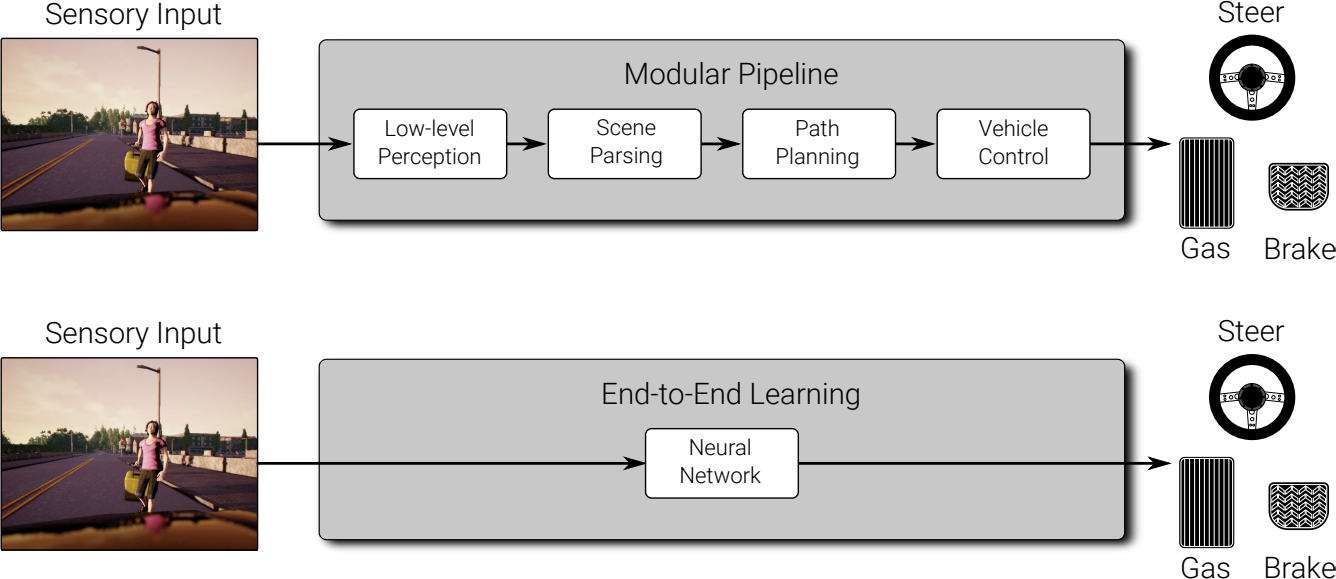
\includegraphics[width=\textwidth]{figures/2/modular-end-to-end.png}
    \caption{Figure showing the difference between modular (top) and end-to-end (bottom) approaches to autonomous vehicles. Source: \cite{computer-vision-for-autonomous-vehicles}.}
    \label{fig:modular-vs-end-to-end}
\end{figure}

As discussed in a recent paper comparing end-to-end techniques, there is an ongoing shift towards the latter approach \cite{survey-on-end-to-end-techniques}. Even though the modular approach offers an explainable and verifiable system where each module can individually be evaluated, it lacks efficient use of computer resources and awareness of the high-level task that is autonomous driving. In addition, the modular approach requires huge amount of annotated data for each module. This is in contrast to the end-to-end approach where the annotations lives in the state of the car (steering commands, GPS location, etc.) at a given moment. This approach does however require the sensors to be synchronized. 


% \section{Challenging Tasks in Autonomous Driving}
% or just "Challenges in Autonomous Driving"

%\subsection{Lane Prediction}
%...

%\subsection{Multi-modal sensors}
%...

\section{Related Work}
\label{sec:related-work}

\subsection{TransFuser (2021)}
TransFuser, ranked 2nd when published and currently ranked 4th on the CARLA Leaderboard,
is an end-to-end approach to autonomous driving in the CARLA simulator
\cite{transfuser-pami, transfuser-cvpr, pwc-carla}.
In their paper, \textcite{transfuser-pami} explores how complementary sensors should be integrated for autonomous driving. Their model uses both RGB images and LIDAR data, and outputs position waypoints that are passed to a traditional PID-controller for steering.
By interleaving Transformer-blocks within both the RGB and LIDAR feature extraction branches,
features are fused between the two sensor modalities leading to exchange of information and supposed improved understanding of the environment. An overview of the architecture is shown in \cref{fig:transfuser-architecture}.

\begin{figure}[htbp]
    \centering
    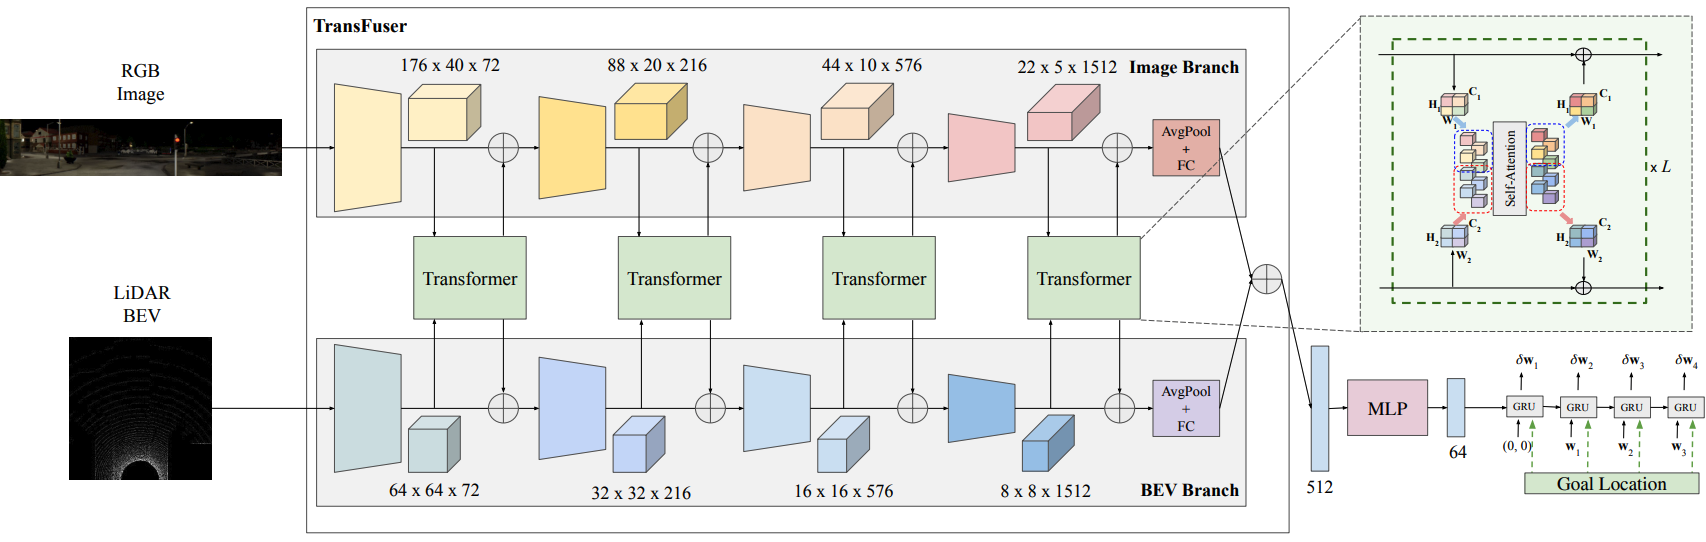
\includegraphics[width=\textwidth]{figures/2/transfuser-architecture.png}
    \caption{The TransFuser architecture uses several transformer modules for the fusion of intermediate feature maps between RGB and LIDAR data. The two branches are combined and fed into an MLP before passing it to an auto-regressive waypoint prediction network.  Source: \cite{transfuser-pami}.}
    \label{fig:transfuser-architecture}
\end{figure}

During training, TransFuser optimizes a multi-task loss consisting of not only predicting waypoints,
but also predicting depth and semantic segmentation images,
as well as a top-down HD-map and bounding boxes vehicle detection.

\textcite{transfuser-pami} also propose a new benchmark for autonomous driving called \textit{Longest6}. This involves longer routes, increased traffic density and more challenging pre-crash scenarios than existing closed-loop driving benchmarks. Another advantage of this benchmark over the official CARLA Leaderboard is that it can be used for evaluation on local resources without the online platform's computation budget restrictions.

As this specialization project is based on the TransFuser model, a more detailed description can be found in  \cref{sec:transfuser}.


\subsection{Learning from All Vehicles (2022)}
\textcite{chen2022lav} presents in their paper a system to train models for autonomous driving on data not just from the ego-vehicle itself, but also other vehicles it observes.
They argue that training on other vehicle's trajectories will help with sample efficiency, greatly increase the chance that the model sees interesting scenarios and help the ego-vehicle avoid collisions. Finding these trajectories are however challenging due to partial observability and the lack of sensors in other vehicles.

\begin{figure}[htbp]
    \centering
    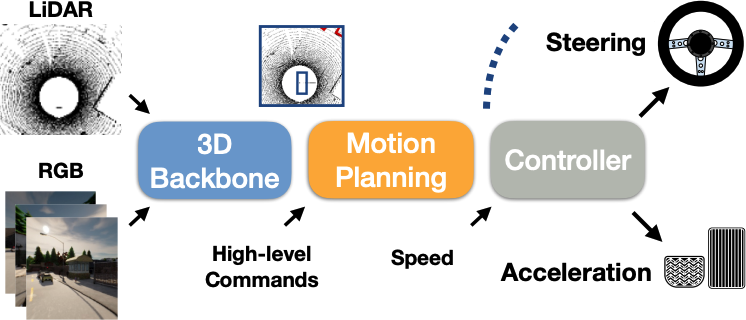
\includegraphics[width=.7\textwidth]{figures/2/lav.png}
    \caption{An overview of the Learning from All Vehicles inference architecture. It consists of three modules: A perception module, a motion planner and a low-level controller. Source: \cite{chen2022lav}.}
    \label{fig:lav}
\end{figure}

Their end-to-end model consists of a three-stage modular pipeline, as seen in \cref{fig:lav}. The first stage is a perception module that maps raw sensor readings from three front-facing RGB cameras and LIDAR to map-view feature representations. Its goal is to create a robust and generalizable representation of the surrounding world, and to build vehicle-invariant features that help supervise the motion planner. The motion planner is the second stage and it uses these features to produce a series of waypoints describing the future trajectory of all vehicles that surrounds the ego-vehicle. The last stage is a low-level controller that converts motion plans into actions to be executed on the vehicle. \textcite{chen2022lav} reached the top of the CARLA Leaderboard with their submitted paper, and is currently ranked 3rd \cite{chen2022lav, pwc-carla}.


\subsection{InterFuser (2022)}
\textcite{shao2022interfuser} propose InterFuser, a safety-enhanced autonomous driving framework. They investigate methods for multi-modal sensor fusion in a more scalable and effective way than TransFuser's multi-stage approach. They also work towards interpretability of their end-to-end model by creating a safety mind map based on immediate features, which they argue can help unveil the model's decision basis and failure causes.

\begin{figure}[htbp]
    \centering
    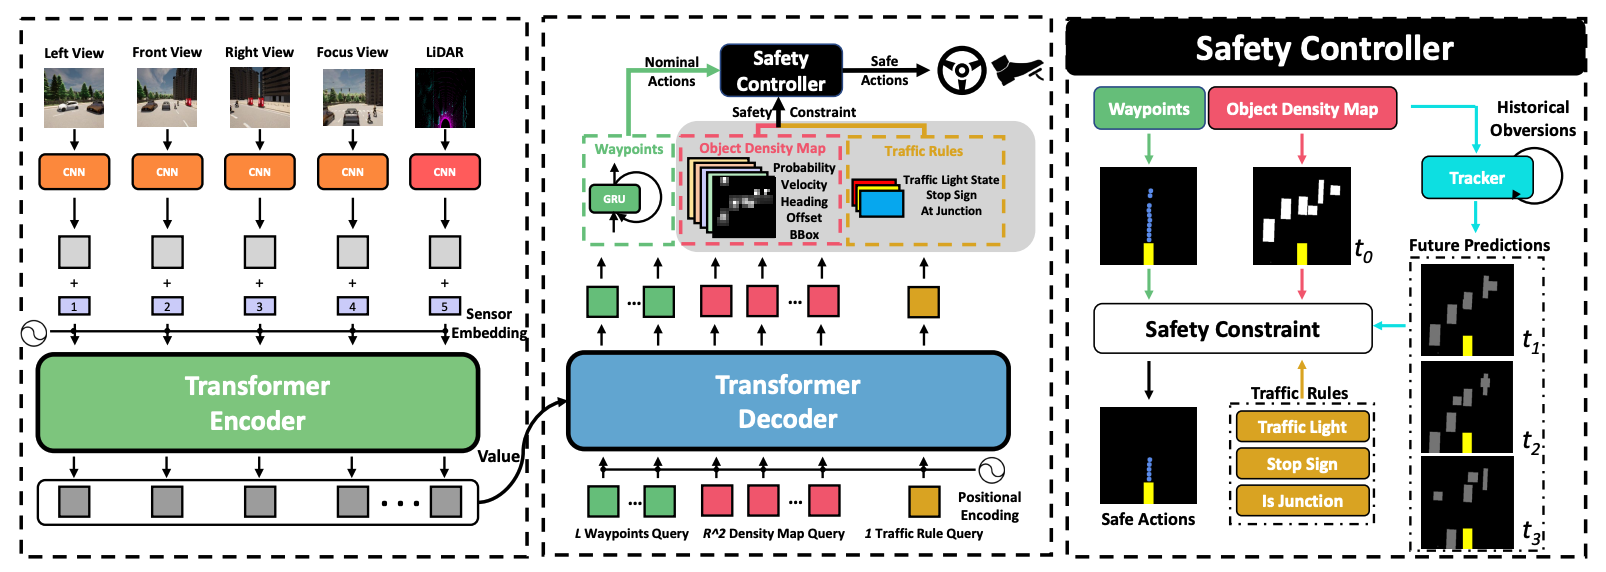
\includegraphics[width=\textwidth]{figures/2/interfuser.png}
    \caption{The InterFuser architecture. It consists of an encoder-decoder network built on transformers, in addition to a safety controller that constraints the output actions to enhance driving safety. Source: \cite{shao2022interfuser}.}
    \label{fig:interfuser}
\end{figure}

The models follows an encoder-decoder architecture as seen in \cref{fig:interfuser}. The input consists of three RGB cameras (left, front and right) and LIDAR. From the RGB cameras they create four images, one for each direction and one focusing-view image to capture distant traffic lights. The inputs are then fused in a multi-view multi-modal transformer before being fed into the decoder. The decoder takes queries in the form of waypoints, density maps and a traffic rule to the attention mechanism and outputs predictions of the same attributes. Finally, a safety controller uses the predicted waypoints, object density map and traffic rule to create a safety mind map, which is utilized to constrain the actions into a safe set. InterFuser is currently the top performer on the CARLA Leaderboard \cite{shao2022interfuser, pwc-carla}.


%InterFuser uses a one-stage architecture to fuse information from multi-modal multi-view sensors, a method they claim is more scalable and effective than TransFuser's multi-stage architecture.
